

% 1 theory 2 deep learning or reverse 3 General machine learning: core contributions in supervised and unsupervised methods 4 Language and multimodal language models

% what we do
Large language models (LLMs) exhibit a striking robustness to surface-level variation. Prompts that differ substantially in wording, style, or syntactic structure often lead to similar internal reasoning and consistent outputs. This behavior suggests that LLMs encode semantic information in a stable internal representation that abstracts away from lexical form. However, despite extensive empirical success, it remains unclear where such stable semantic representations emerge within model architectures, how they can be formally characterized, and how their geometric structure differs across models.

\begin{figure}[h]
    \centering
    \vspace{-0.75em}
    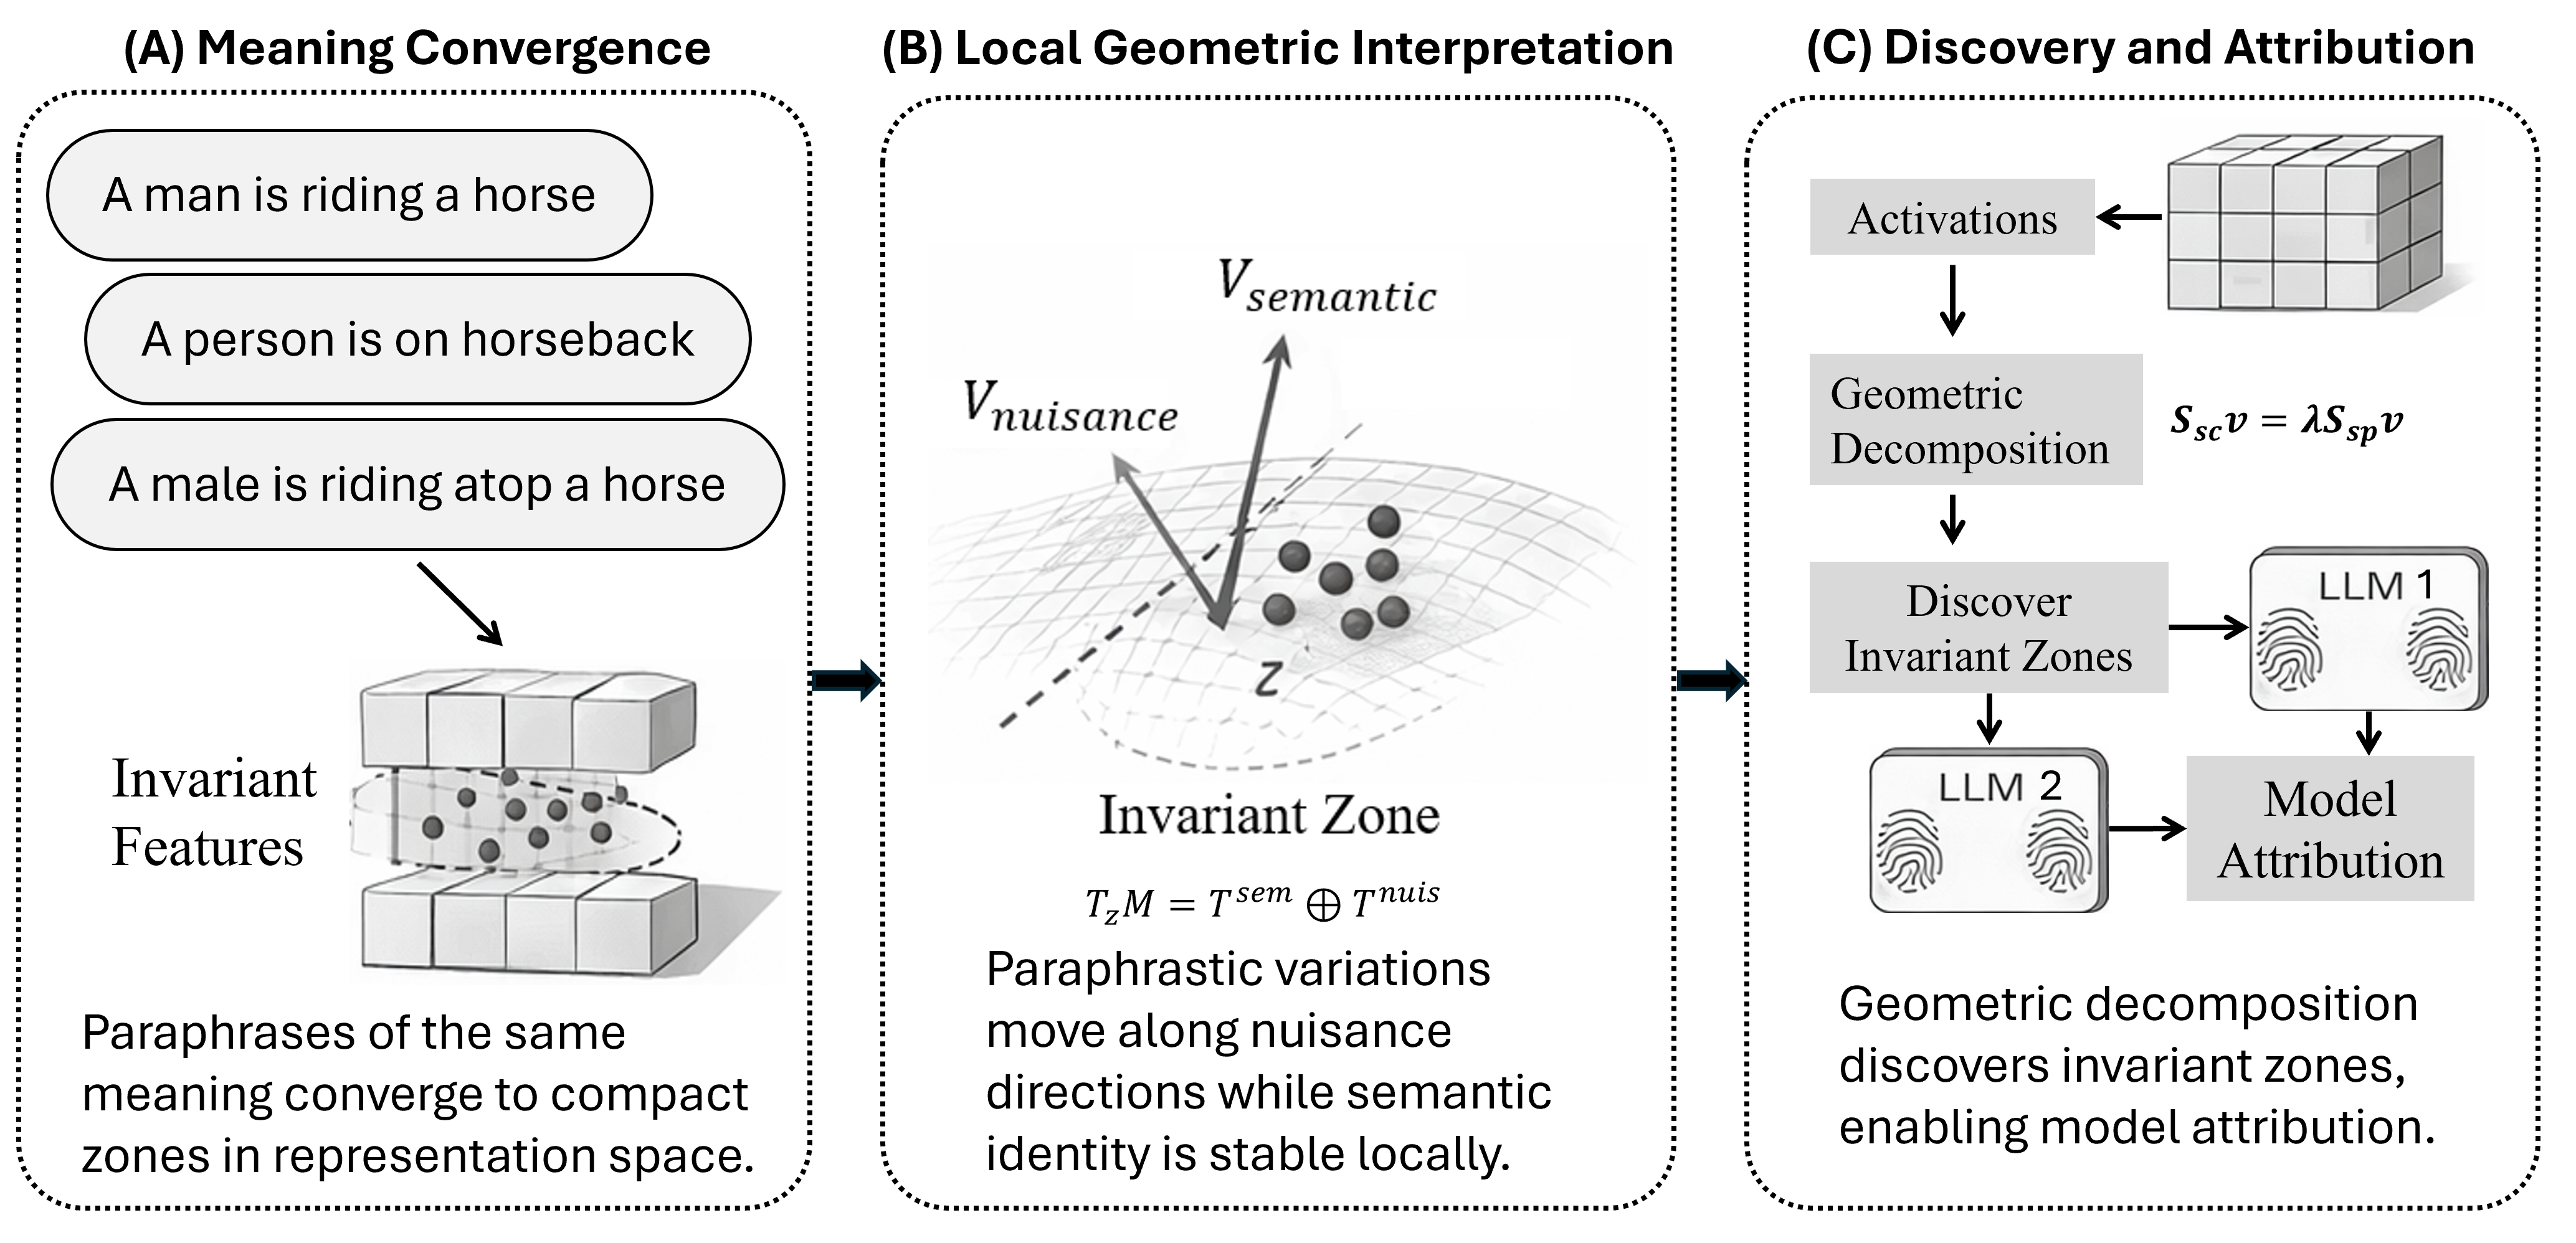
\includegraphics[width=0.9\linewidth]{figures/1_PIA.png}
    \vspace{-0.75em}
    \caption{Emergence of invariant semantic regions in LLMs. (A) Paraphrases propagate through layers and tend to converge to compact zones.
    (B) Local geometric interpretation: nuisance vs semantic tangent directions.
    (C) Geometric decomposition detects invariant zones for model attribution.}
    \label{fig:FIA}
    \vspace{-1.5em}
\end{figure}

% why we need it
Understanding invariant internal representations is important for both scientific and practical reasons. From a representation learning perspective, identifying where semantic stability arises provides insight into how transformers organize meaning across depth and how abstraction emerges during inference. From a systems and security perspective, invariant representations offer a mechanism to analyze model behavior beyond observable outputs. Because these internal structures reflect how a model organizes semantic information, they may support applications such as model attribution, forensic analysis, and robustness evaluation.

% current summary
Existing efforts to analyze or identify language models span several complementary directions. Prior work on semantic representations and probing has shown that transformer activations encode structured linguistic and semantic information and exhibit robustness to paraphrasing. A separate line of work studies representation geometry through similarity metrics and subspace analysis, revealing that learned features admit meaningful low-dimensional structure across layers and models. More recently, model attribution and fingerprinting approaches have demonstrated that internal activations and outputs can contain model-specific signals. 
While these studies provide important insights, they largely treat semantic stability, representation geometry, and model identity as separate phenomena. In particular, existing approaches do not provide a local geometric characterization of semantic invariance as a structural property of latent representations, nor a principled mechanism to identify invariant structure by explicitly separating semantic-preserving and semantic-changing variation. As a result, it remains difficult to systematically understand how semantic invariance emerges across layers and how it relates to model-specific representation geometry.

In this work, we develop a geometric framework for analyzing semantic invariance in language models. As illustrated in Fig.~\ref{fig:FIA}, we hypothesize that semantically equivalent inputs form locally stable regions in latent space, where semantic-preserving and semantic-changing variations correspond to approximately distinct nuisance and semantic directions. 
(1) Building on this hypothesis, our first contribution is a local geometric definition of invariant latent features as representations that are stable under semantic-preserving transformations while remaining discriminative across meanings. 
(2) Our second contribution is a data-driven framework for identifying local invariant features via contrastive sensitivity decomposition, which separates semantic-changing from semantic-preserving variation.
(3) Our third contribution is to show that these invariant zones exhibit model-specific geometry and can serve as latent signatures for zero-shot model attribution, demonstrating that invariant representations encode both semantic stability and model individuality. 

